
\section*{Общая характеристика работы}

\newcommand{\actuality}{\underline{\textbf{\actualityTXT}}}
\newcommand{\progress}{\underline{\textbf{\progressTXT}}}
\newcommand{\aim}{\underline{{\textbf\aimTXT}}}
\newcommand{\tasks}{\underline{\textbf{\tasksTXT}}}
\newcommand{\novelty}{\underline{\textbf{\noveltyTXT}}}
\newcommand{\influence}{\underline{\textbf{\influenceTXT}}}
\newcommand{\methods}{\underline{\textbf{\methodsTXT}}}
\newcommand{\defpositions}{\underline{\textbf{\defpositionsTXT}}}
\newcommand{\reliability}{\underline{\textbf{\reliabilityTXT}}}
\newcommand{\probation}{\underline{\textbf{\probationTXT}}}
\newcommand{\contribution}{\underline{\textbf{\contributionTXT}}}
\newcommand{\publications}{\underline{\textbf{\publicationsTXT}}}


% Обзор, введение в тему, обозначение места данной работы в
% мировых исследованиях и~т.\:п., можно использовать ссылки на~другие
% работы\cite{Joshi2015}
% % (если их~нет, то~в~автореферате
% автоматически пропадёт раздел <<Список литературы>>). Внимание! Ссылки
% на~другие работы в разделе общей характеристики работы можно
% использовать только при использовании \verb!biblatex! (из-за технических
% ограничений \verb!bibtex8!. Это связано с тем, что одна
% и~та~же~характеристика используются и~в~тексте диссертации, и в
% автореферате. В~последнем, согласно ГОСТ, должен присутствовать список
% работ автора по~теме диссертации, а~\verb!bibtex8! не~умеет выводить в одном
% файле два списка литературы).
% При использовании \verb!biblatex! возможно использование исключительно
% в~автореферате подстрочных ссылок
% для других работ командой \verb!\autocite!, а~также цитирование
% собственных работ командой \verb!\cite!. Для этого в~файле
% \verb!Synopsis/setup.tex! необходимо присвоить положительное значение
% счётчику \verb!\setcounter{usefootcite}{1}!.

% Для генерации содержимого титульного листа автореферата, диссертации
% и~презентации используются данные из файла \verb!common/data.tex!. Если,
% например, вы меняете название диссертации, то оно автоматически
% появится в~итоговых файлах после очередного запуска \LaTeX. Согласно
% ГОСТ 7.0.11-2011 <<5.1.1 Титульный лист является первой страницей
% диссертации, служит источником информации, необходимой для обработки и
% поиска документа>>. Наличие логотипа организации на титульном листе
% упрощает обработку и поиск, для этого разметите логотип вашей
% организации в папке images в формате PDF (лучше найти его в векторном
% варианте, чтобы он хорошо смотрелся при печати) под именем
% \verb!logo.pdf!. Настроить размер изображения с логотипом можно
% в~соответствующих местах файлов \verb!title.tex!  отдельно для
% диссертации и автореферата. Если вам логотип не~нужен, то просто
% удалите файл с логотипом.

{\actuality}


Начиная с зарождения первых цивилизаций и до сегодняшнего момента вопросы о
том, как устроены сознание и разум в человеке и других живых существах,
продолжают быть для нас ключевыми.  Так сложилось, что их осмысление
происходило сперва в рамках религиозной, а затем и философской парадигмы,
которые в западноевропейской традиции значительно перекликались и дополняли
друг друга.

Научный подход к вопросам познания сформировался лишь относительно недавно в рамках группы
дисциплин, включающей в себя нейробиологию, нейрофизиологию, когнитивную психологию и
электрофизиологию. В рамках этих дисциплин ключевым для понимания когнитивной функции человека
и животных в самом широком смысле становится устройство центральной нервной системы и, в частности,
головного мозга.

Интересно, что механизмы познания связывались с функцией головного мозга не
всегда даже в рамках материалистического описания. Так например, Аристотель
считал источником мысли сердце, а мозгу отводил лишь роль радиатора,
охлаждающего кровь. Тем не менее, уже в эпоху классической античности Гален
сформировал идею о том, что именно мозг является источником мысли, а значит и
тем инструментом, с помощью которого реализуется познание.  На укоренение идеи
о том, что изучение работы центральной нервной системы и её высшего отдела~---
коры больших полушарий~--- способно предложить ответ на фундаментальный вопрос
“что представляет собой человеческий интеллект”, ушло еще более полутора тысяч
лет.  На сегодняшний день удовлетворительного ответа на этот вопрос по-прежнему
нет и появится он, вероятно, не скоро. Однако в ходе  долгого и непростого
движения к этой Ultima Thule наше понимание более прикладных вещей, сопряженных
с нейрофизиологией, несравненно обогатилось.  С практической точки зрения
трудно переоценить значение понимания работы ЦНС для медицины, не
ограничиваясь, однако, лишь ею.

Сегодня, вместе со всеобщим размыванием междисциплинарных границ, нейронауки
все больше оказываются связанными с более техническими и инженерно-прикладными
дисциплинами.  Так, в 1943 году вдохновленные архитектурой нейронных ансамблей
живого мозга Маккаллок и Питтс создают первую вычислительную модель нейронной
сети, породив тем самым столь популярный сегодня класс алгоритмов машинного
обучения~\cite{McCulloch}. Все большую популярность приобретают сегодня
мозг-компьютерные интерфейсы, позволяющие формировать управляющую команду на
основе электромагнитной активности мозга напрямую, что открывает совершенно
новые перспективы для интеграции человека с машиной.

% \section{Модальности изучения активности мозга.}

В этой связи развитие методов, связанных с изучением строения и работы мозга а
также декодирование порождаемых им сигналов представляет сегодня чрезвычайный
интерес.  Вместе с тем, за последние сто лет благодаря резкому скачку в
развитии электроники, физики и компьютерных наук набор инструментов в руках
ученого-нейрофизиолога существенно обогатился.  На сегодняшний день
существующие методы с точки зрения необходимости хирургического вмешательства
для проведения измерений можно разделить на инвазивные и неинвазивные.

К первой группе относится интракраниальная энцефалография~--- метод, в котором
электрические потенциалы записываются напрямую с коры больших полушарий.
Недостатки и преимущества такого подхода очевидны. К первым прежде всего
относится необходимость хирургического вмешательства для проведения измерений,
что существенно ограничивает возможности исследователя-нейрофизиолога в
получении данных для исследования.  На практике осуществление таких измерений
на человеке возможно лишь для пациентов, прошедших операцию на мозге в связи с
каким-либо неврологическим заболеванием, как правило эпилепсией.  В ходе
операции для мониторинга активности мозга после хирургического вмешательства на
кору головного мозга устанавливаются электроды, регистрирующие электрическую
активность.  Ясно, что количество таких данных, как и  возможность проведения
каких-либо сложных когнитивных экспериментов на пациентах, прошедших операцию
на мозге, весьма ограничены.  При этом качество электрического сигнала,
записанного в непосредственной близости от его источника, несравненно выше
того, что можно получить, записывая электроэнцефалограмму с поверхности кожи
головы.

Неинвазивные методы, с другой стороны, представляют собой намного более гибкий
инструмент для исследований головного мозга человека в силу отсутствия
необходимости проведения операции.  Для изучения анатомической организации
мозга а также в качестве вспомогательного инструмента при анализе активности
нейронных популяций коры используются методы структурной нейровизуализации,
такие как магнитно-резонансная томография (МРТ), компьютерная томография (КТ) и
диффузионная тензорная визуализация (ДТВ).  Они позволяют неинвазивно получать
статические трехмерные изображения тканей головного мозга.  Для изучения
динамической активности нейронов используются функциональные методы
нейровизуализации, а именно~---  функциональная магнитно-резонансная томография
(фМРТ), позитронно-эмиссионная томография (ПЭТ), электроэнцефалогафия (ЭЭГ), а
также магнитная энцефалография (МЭГ).

При этом лишь последние два метода измеряют электрическую активность мозга
непосредственно, тогда как фМРТ и ПЭТ меряют локальный кровоток, который
меняется сравнительно медленно, существенно ограничивая временное разрешение
этих методов.  Так, для ЭЭГ и МЭГ временное разрешение оказывается равным
$\approx$ 1мс, а методы, измеряющие локальный кровоток, позволяют разрешить
лишь процессы с характерными временами порядка одной секунды и медленнее.
Вместе с тем, осцилляторные электрофизиологические процессы, порождаемые
тканями головного мозга, имеют характерные времена от 0.1 секунды и быстрее~\cite{buzsaki}.
Таким образом, среди
всех имеющихся на сегодняшний день инструментов анализа,
\emph{только ЭЭГ и МЭГ позволяют осуществлять неинвазивные записи сравнительно быстрой
электрофизиологической активности головного мозга}, что делает их незаменимым
инструментом при изучении \emph{осцилляций} и их \emph{синхронизации} в головном
мозге человека.

% \section{Осцилляции и их роль в обмене информацией между популяциями нейронов.}

Способность порождать осцилляции или ритмическую токовую активность является
существенной чертой, присущей работе нейронных популяций. Природа возникающих
ритмов, а также их функциональное назначение на сегодняшний день остаются
предметом изучения, и нет единой, принятой всеми точки зрения на этот счет.
Однако, широко принимается гипотеза, согласно которой осцилляции, порождаемые
различными нейронными популяциями, служат механизмом, позволяющим различным
функционально-специфичным областям мозга избирательно осуществлять обмен
информацией друг с другом. Иными словами, предполагается, что осцилляции
ответственны за процессы \emph{функциональной интеграции}.
%~\cite{TODO}.

Согласно существующим представлениям, функциональная интеграция нейронных
ансамблей осуществляется за счет синхронизации порождаемых этими ансамблями
осцилляций. При этом области коры, в которых ритмическая активность
синхронизована, получают возможность эффективнее передавать информацию, а
десинхронизованные области, напротив, перестают обмениваться сигналами. Такое
представления об организации эффективных каналов передачи информации между
нейронными ансамблями за счет синхронизации получило в литературе название
<<взаимодействие через когерентность>> (в английском варианте communication
through coherence, CTC)~\cite{Fries2015}. Иными словами, синхронизация
осцилляций являются тем механизмом, который позволяет динамически связывать в
сети функционально специфичные области мозга для выполнения определенной
когнитивной задачи. Изучение таких сетей, возникающих и распадающихся в
процессе решения мозгом определенных когнитивных задач, является сегодня одной
из центральных тем в изучении мозговой активности, как в норме, так и при
патологии~\cite{varela, baker, ossadtchi, Bastin2017},~\cite{Alamian_front2017,
Alamian_clin2017}

С точки зрения исследования таких сетей выделяют понятие \emph{функциональной
коннективности}, понимая под этим статистические закономерности в одновременной
активации (в самом широком смысле) различных областей мозга.
%~\cite{TODO}.
При этом вывод о том, что эти области мозга работали синхронно, делается на
основании вычисления определенной метрики, отражающей степень сходства
измеренных (или математически восстановленных) в этих областях сигналов.  Такие
метрики называются \emph{мерами коннективности}.

Многое в области изучения функциональной коннективности было сделано с
использованием технологии фМРТ, однако отмеченное выше ограничение фМРТ в виде
плохого временного разрешения делает электрофизиологические методы измерений
незаменимыми при анализе коннективности. Особое место при этом занимает
магнитная энцефалография, которая в сочетании с методами восстановления сигнала
на коре головного мозга в силу более высокой точности прямой модели по
сравнению с ЭЭГ предоставляет в руки исследователя уникальное сочетание менее
чем сантиметрового разрешения по пространству и миллисекундного разрешения по
времени~\cite{hamalainen, Baillet, Gross2013}.


% \section{Существующие методики поиска синхронных осцилляций.}

% {\progress}
Вообще, оценка коннективности на основании неинвазивных электрофизиологических
данных, представляет собой сложную инженерную задачу, на решение которой
научное сообщество уже потратило немало сил.  За последние несколько
десятилетий было разработано и опробовано множество методов оценки
функциональной коннективности от стандартных подходов, включающих меры
синхронизации сигналов во временной и частотной области (таких как корреляция и
когеренция), до более изощренных, зачастую нелинейных мер
коннективности~\cite{Marzetti2008, Schoffelen2009, Colclough2015, kaminski,
greenblatt_conn, hillebrand, imcoh, Lachaux1999, env_corr, Brookes2012,
Brookes2011, Hillebrand2012, Hipp2012, PLI, wPLI, Chella2015, Chella2016,
Wibral2011, Ioannides2000}.  Ни одна из предложенных мер, обладая своими
достоинствами и недостатками, не является, однако, универсальной в силу
сохраняющихся технических затруднений~\cite{Colclough2016, Bastos2016}.

Одной из наиболее существенных проблем, возникающих при оценке функциональной
коннективности является так называемая \emph{протечка сигнала}, объясняемая
тем, что обратная задача для ЭЭГ/МЭГ является некорректной. Практически это
означает, что имея ограниченный набор измерений нельзя однозначно восстановить
конфигурацию источников, породивших сигнал. Из этого, в свою очередь, следует
невозможность полностью размешать сигналы, записанные сенсорами,~--- в каждый
из восстановленных сигналов неизбежно будут подмешаны сигналы от остальных
источников. Следовательно, все восстановленные сигналы будут в какой-то степени
похожи друг на друга, даже если исходные сигналы не демонстрировали никаких
признаков синхронизации. А значит и меры коннективности, будучи мерами сходства
сигналов, будут демонстрировать завышенные значения.
Возникает проблема различения
истинной синхронности и той, которая порождена фундаментальными ограничениями
неинвазивной электрофизиологии.

Впервые попытка решения этой проблемы была предпринята в 2004 году в статье Г.
Нолте~\cite{imcoh}, в которой авторы предлагают использовать в качестве меры
коннективности величину, называемую мнимой частью когеренции.  Для этого каждый
сигнал сначала необходимо перевести в частотную область, затем для каждой пары
сигналов посчитать функцию когерентности, и наконец, взять от полученной
величины её мнимую часть.  Идея такого метода оценки коннективности заключается
в том, что мнимая часть когеренции имеет ненулевое значение лишь для сигналов с
ненулевой разностью фаз, тогда как эффект протечки сигнала всегда проявляется в
виде ложной синхронизации с нулевой фазовой задержкой, давая тем самым вклад
лишь в действительную часть когеренции. Действительно, такой подход существенно
повышает устойчивость метода к протечке сигнала. Тем не менее, так как функция
когерентности нормируется на оцененные мощности сигналов (которые, будучи чисто
действительными величинами, подвержены влиянию протечки сигнала) итоговые
оценки коннективности по мнимой части когеренции также, пусть и в меньшей
степени, испорчены эффектом протечки.

На эту деталь в 2007 году обратил внимание Стэм в своей статье~\cite{PLI}.
Стэм предложил использовать для оценки синхронизации
вместо мнимой части когеренции среднее значение знака разности фаз двух сигналов.
Такая мера оказывается очень похожей на мнимую часть когеренции, однако нормировка
(скрытая в операции взятия знака мнимой части) теперь производится лишь на чисто мнимые величины, которые не
зависят от протечки сигнала. Стэм назвал свою меру индексом фазовой задержки (phase lag index, PLI).

Следующей ступенью эволюции в цепочке методов, основанных на идее мнимой части когеренции стала
мера, называемая взвешенным индексом фазовой задержки (weighted phase lag index, wPLI). Ее описал Винк с
соавторами в своей статье 2011 года. Мотивацией к разработке новой меры коннективности послужил тот
факт, что мера PLI оказалась слишком неустойчивой по отношению к шуму. Основной недостаток индекса фазовой
задержки, как и его преимущество перед мнимой частью когеренции, кроется в операции взятия знака.
Дело в том, что для шумовых источников случайно меняющийся знак разности фаз оказывает слишком большое
влияние на измерения. Чтобы избавиться от этого недостатка, Винк предложил взвешивать знак разности фаз
на амплитуду мнимой части соответствующих кросс-спектральных коэффициентов. Таким образом, вклад от шумовых
источников малой амплитуды оказывается малым, что делает меру более устойчивой.

Семейство мер коннективности, основанных на мнимой части когеренции, не
исчерпывается обозначенными тремя подходами. Аналогичная идея, но под немного
другим углом, была применена в статье~\cite{Hipp2012} 2012 года. В ней в
качестве меры синхронности авторы используют корреляцию огибающих двух
узкополосных сигналов. Проблема протечки сигнала в статье решена следующим
образом: на коре восстанавливаются два временных ряда, затем один из них
проецируется ортогонально второму, после чего вычисляются огибающие и
рассчитывается коэффициент корреляции между ними.  Такой подход, основанный на
ортогонализации временных рядов, оказывается эквивалентным взятию мнимой части
соответствующего кросс-спектрального коэффициента.


% TODO: Еще можно написать про wedge music

Все изложенные методики, основанные на мнимой части когеренции, имеют, однако,
один существенный недостаток, а именно~--- все они не чувствительны к
синхронизации с нулевой фазовой задержкой. Как уже отмечалось выше, операция
взятия мнимой части когеренции эквивалентна удалению из данных профилей
синхронизации с нулевой фазовой задержкой. Практически это означает не только
невозможность детектирования сетей, синхронизированных с нулевой фазой, но и
плохое отношение сигнал / шум (ОСШ) для сетей, для которых фазовая задержка
мала. Более того, чем ближе эта фазовая задержка к нулю, тем хуже ОСШ для отдельно взятой пары
источников.
И наоборот, чем разность фаз двух сигналов ближе к $\pi / 2$, тем выше значение ОСШ.

Ясно, что такое неравномерное распределение детекторных характеристик метода по
фазовым задержкам ограничивает возможности исследователя.
Этот факт усугубляется тем, что
синхронизация с нулевой фазой, по всей видимости, является широко представленным
явлением в организации осцилляторной мозговой активности,~\cite{roelfsema, Singer1999, Engel2001},
которое может быть объяснено наличием общего входа для двух узлов сети, либо
их двунаправленным взаимодействием,~\cite{rajagovindan}.

По этой причине на сегодняшний день в неинвазивной электрофизиологии имеется
острая потребность в появлении иснструмента измерения коннективности, который,
с одной стороны, будет устойчив к эффекту протечки сигнала, а с другой~---
будет способен обнаруживать сети для всего спектра фазовых задержек.


Попытка создать такой метод была предпринята в 2015 году в
статье~\cite{Wens2015}. В ней авторы использовали принципиально иной метод
борьбы с эффектом протечки сигнала.  Идея этого метода состоит в использовании
информации о взаимном расположении источников сигнала и сенсоров для
конструкции особых пространственных фильтров, которые позволяют очистить один
источник от сигнала, пришедшего от другого источника для последующего измерения
какого-либо индекса синхронности. Авторы в качестве такого индекса предложили
использовать корреляцию огибающих сигналов. Более детально структура
предложенного метода такова. Во-первых, по сигналам на сенсорах
восстанавливаются сигналы на источниках.  Далее фиксируется один из источников
на коре.  Все остальные источники пространственно фильтруются от активности,
протекшей от фиксированного источника.  Далее меряется корреляция огибающих
между фиксированным источником и всеми остальными.  Чтобы получить значение
коннективности для каждой пары источников нужно повторить процедуру, выбирая в
качестве фиксированного источника каждый из оставшихся.  Наконец, так как
полученная матрица коннективностей будет вообще говоря асимметричной, значения
значения коннективности для пар $(i,j)$ и $(j,i)$ усредняются. Такую эвристику
авторы статьи назвали методом геометрической поправки (geometric correction
scheme, GCS).

Метод GCS концептуально явился серьезным продвижением вперед, так как теперь
появилась возможность детектировать сети малыми сдвигами фаз оставаясь (по
крайней мере, в теории) вне влияния эффекта протечки сигнала.  В
действительности однако, такой метод коррекции лишь частично нивелирует
негативный эффект протечки, так как он не учитывает протечку от третьих
источников при оценке коннективности. В качестве примера можно рассмотреть ситуацию, когда имеется
три мощных источника, никакие два из которых не были синхронизированы.  В такой
постановке, несмотря на отсутствие синхронностей, метод GCS покажет высокие
значения коннективности для всех трех пар связей, так как хотя для каждой пары
коррекция очистит сигналы от протечки друг в друга, сигнал от третего
источника, протекая в каждый источник из пары, создаст общую компоненту в
восстановленных источниках.  В результате коннективность, которую мы измерим
для исходно не синхронных источников, после геометрической коррекции для пары
источников фактически будет отражать степень протечки от третьего источника в
каждый сигнал из пары. Ясно, что если третий сигнал лежит близко к первым двум,
эффект протечки будет весьма существенным. В результате для большого количества
активных источников даже очищенный сигнал оказывается крайне загрязненным, что
существенно ограничивает применимость GCS к практическим задачам.


Таким образом, \emph{до сих пор не существует метода оценки коннективностей,
позволяющего надежно детектировать сети с малыми фазовыми задержками и при этом свободного
от эффекта протечки сигнала.}


% \section{Оценивание функциональной коннективности в условиях некорректности обратной задачи М/ЭЭГ.}\label{sec:connectivity_and_ill_posedness}

Современная практика использования мер коннективности в нейрофизиологических
исследованиях в подавляющем большинстве случаев следует одной из двух возможных схем.
Первая схема предполагает изучение нейрофизиологического эффекта  в \emph{пространстве сенсоров},
т.е. выбранная исследователем мера коннективности применяется непосредственно к сигналам,
записанным электродами.
Второй вариант предполагает переход в пространство источников~--- сначала оцениваются
возможные источники записанной электрофизиологической активности на коре, а затем к этим
источникам применяется та или иная  мера коннективности.

Очевидным образом, первый вариант позволяет дать лишь весьма грубую оценку локализации
узлов восстановленных сетей, поэтому часто используется лишь как первое приближение к результату.
Более интересным, хотя и более сложным концептуально и более
трудоемким с точки зрения вычислительных ресурсов, является второй вариант, в котором
сначала оценивается сигнал на источниках, а потом считается мера коннективности.

Оценка источников в неинвазивной электрофизиологии является
некорректной обратной задачей~\cite{Hamalainen1993}:
ее решение не определено однозначно. Иными словами, любые электрофизиологические измерения,
сделанные ограниченным набором сенсоров, можно объяснить бесконечным количеством конфигураций
источников электромагнитной активности, расположенных на коре. Подавляющее большинство таких конфигураций
при этом будет абсурдным с точки зрения физиологии. Среди бесконечного набора
решений необходимо выбрать то, которое с одной стороны хорошо объясняет наблюдения, а с другой~---
соответствует имеющимся представлениям о физиологии мозга.

Поэтому решение обратной задачи в неинвазивной электрофизиологии всегда требует
внедрения в модель дополнительной априорной информации о структуре решения. Не
в каждом методе решения обратной задачи можно явно указать тот момент, в
который делается дополнительное предположение о структуре решения, однако
большая часть таких методов (например,~\cite{Hamalainen1994, Uutela1999, Pascual-Marqui1994, Pascual-Marqui2002})
может быть описана в терминах Тихоновской регуляризации~\cite{tikhonov},
позволяющей свести задачу поиска решения к минимизации
функционала, состоящего из двух членов: первый определяет, насколько хорошо решение
объясняет измеренный сигнал, а второй~--- насколько оно соответствует тому классу
решений, который мы считаем <<физиологичным>>. При этом, формализация понятия
<<физиологичный>> может включать в себя широкий спектр различных предположений
о структуре решения~--- от естественного требования непрерывности по
пространству и времени (как в MNE,~\cite{Hamalainen1994}) до требования соответствия
инидивидуально восстановленной анатомической структуре нейрональных связей.

Оценка источников в такой постановке происходит оптимально с точки зрения минимизации
выбранного функционала, однако в задаче поиска синхронных осцилляций оценка источников не
является самоцелью. Оптимальность этой оценки не гарантирует оптимальности оценки
достаточных статистик синхронности в пространстве источников.

% TODO
Двухступенчатая процедура оценки коннективностей в общем случае
дает субоптимальные результаты с точки зрения оценивания соответствующих статистик.
% Ситуация здесь может быть улучшена рассмотрением порождающих моделей для этих статистик статистик.
% В данной работе такой подход изложен в применении к матрице \emph{кросс-спектральной плотности},
% являющейся достаточной статистикой для оценки фазовой синхронности в
% пространстве источников \cite{cross_sufficient}.
Оптимальное оценивание по наблюдениям для статистик синхронности в пространстве источников требует
рассмотрения порождающих моделей с формулировкой априорных посылок для сетей вместо таковых для
источников. В частности, желательно было бы находить такие решения обратной задачи, которые
объясняют измерения \emph{минимальным набором сетей}. Мотивация такого подхода кроется в известном
принципе бритвы Оккама~--- объяснение наблюдаемых данных должно быть максимально простым.
Известно, что решения такого вида, то есть те, в которых число отдельных структурных элементов,
объясняющих данные, минимально, реализуются при помощи спарсной регуляризации.
Как вводить такую регуляризацию в рамках двухступенчатой процедуры, однако, не совсем
понятно.



 % \ifsynopsis
% Этот абзац появляется только в~автореферате.
% Для формирования блоков, которые будут обрабатываться только в~автореферате,
% заведена проверка условия \verb!\!\verb!ifsynopsis!.
% Значение условия задаётся в~основном файле документа (\verb!synopsis.tex! для
% автореферата).
% \else
% Этот абзац появляется только в~диссертации.
% Через проверку условия \verb!\!\verb!ifsynopsis!, задаваемого в~основном файле
% документа (\verb!dissertation.tex! для диссертации), можно сделать новую
% команду, обеспечивающую появление цитаты в~диссертации, но~не~в~автореферате.
% \fi

% Этот раздел должен быть отдельным структурным элементом по
% ГОСТ, но он, как правило, включается в описание актуальности
% темы. Нужен он отдельным структурным элементом или нет ---
% смотрите другие диссертации вашего совета, скорее всего не нужен.
Имея в виду все вышесказанное, можно заключить, что на сегодняшний день
процедура оценки коннективности по неинвазивным электрофизиологическим данным с одной стороны
все еще является плохо разработанной и нуждается в улучшениях (неслучайна
регулярная публикация новых методологических статей по теме оценки коннективностей),
а с другой является ключевым инструментом для современной нейрофизиологии,
следуя за смещением акцента в изучении мозга от активации его отдельных областей к взаимодействию
между ними.

{\aim} данной работы, таким образом, является разработка метода
оценки коннективностей, который
\begin{itemize}
        \item позволяет оценить фазовую синхронность в условиях взаимной протечки сигналов
        \item чувствителен к сетям с малыми фазовыми задержками
        \item оптимален с точки зрения оценки достаточной статистики для коннективности
        \item способен учитывать априорную информацию об организации фазовых синхронностей
        \item не чувствителен к протечке сигнала на уровне сетей
\end{itemize}
а также его валидация в применении к симуляционным МЭГ-данным.

Для~достижения поставленной цели необходимо было решить следующие {\tasks}:
\begin{enumerate}
  \item Разработать методику очистки сигнала от протечки сигнала
  \item Исследовать свойства методики очистки сигнала
        для сетей с малым и большим фазовым сдвигом;
        сравнить с методиками, описанными в литературе.
  \item Разработать методологию оптимального оценивания достаточной статистики
        для фазовых синхронностей.
  \item Реализовать алгоритм оценивания, позволяющий использовать спарсную регуляризацию
  \item Разработать код для численного решения задачи невыпуклой оптимизации
  \item Разработать методику визуализации найденных сетей.
  \item Разработать методологию генерации данных, симулирующих мозговую активность
  \item Сравнить детекторные характеристики разработанного метода на симуляционных данных
        по стандартным метриках (AUC-ROC, AUC-Pre-Rec)
\end{enumerate}


{\novelty}
\begin{enumerate}
  \item Впервые задача оценки коннективностей была рассмотрена в пространстве пар источников.
  \item Впервые была продемонстрирована возможность очистки сигнала от эффекта протечки
        при помощи операции ортогональной проекции.
  \item Впервые был сформулирован критерий оптимальной очистки от протечки сигнала
      для оценки фазовой синхронизации.
  \item Впервые задача оценки матрицы кросс-спектральной плотности в пространстве источников
        была решена методом глобальной оптимизации.
\end{enumerate}

{\influence}
Теоретическая значимость определяется тем, что
впервые предложен подход к борьбе с проблемой протечки
сигнала через векторизацию порождающей модели кросс-спектра,
а также с помощью методов оптимальной фильтрации и глобальной оптимизации.

Практическая значимость состоит в том, что разработанный набор алгоритмов
предоставляет новый инструмент в руки исследователя-электрофизиолога. Этот
инструмент позволяет изучать взаимодействия корковых структур, ранее
доступные для изучения только инвазивными методами.

{\methods}
Исследования основаны на теории обратных задач, теории оценивания,
методах цифровой обработке сигналов, оптимальной фильтрации,
глобальной оптимизации невыпуклых функций, а также на работах
по методам оценки фазовой связности в электрофизиологии.

{\defpositions}
\begin{enumerate}
  \item Разработан метод, позволяющий обнаруживать связанные по фазе источники с околонулевыми фазовыми задержками
      по неинвазивным МЭГ-записям. Суть метода заключается в построении пространственного фильтра,
      действующего в пространстве векторизованных матриц кросс-спектральной плотности мощности,
      который позволяет подавить вклад членов, ответственных за эффект протечки сигнала, маскирующий
      информацию о взаимодействии с околонулевой фазой.
  \item Показана оптимальность предложенного фильтра с точки зрения удаления вклада третих источников
      в оценку фазовой связности для фиксированной сети.
  \item На основе метода глобальной оптимизации IrMxNE и предложенного фильтра разработан метод,
      устойчивый к протечке сигнала на уровне сетей и на уровне источников. Первое обеспечивается
      спарсными свойствами метода IrMxNE, второе~--- свойствами разработанного фильтра.
\end{enumerate}

{\reliability} полученных результатов обеспечивается теоретическими выкладками, результатами численного моделирования,
сравнении с другими методами оценки фазовой связности, а также
валидацией разработанного метода на реальных данных.

{\probation}

Основные результаты работы докладывались~на:
\begin{enumerate}
    \item Международная конференция ``Methodological problems of cortex regions functional synchronisation assessment based on MEG/EEG data'',\\
      Тема: \emph{Globally-optimized power and shift invariant imaging of coherent sources (GO-PSIICOS)}\\
      Москва, Россия, 2015.
    \item Международная конференция ``Brain Connectivity Workshop 2015'', \\
        Тема: \emph{GO-PSIICOS (Globally-Optimized Power and Shift Invariant Imaging of Coherent Sources)},\\
        Сан Диего, США, 2015.
    \item Международная конференция ``Biomag 2016'', \\
        Тема: \emph{Power and shift invariant imaging of coherent sources by MEG data},\\
        Сеул, Южная Корея, 2016.
    \item Международная конференция ``Biomag 2018'', \\
        Тема: \emph{Oblique projection for phase shift invariant imaging of coherent sources},\\
        Филадельфия, США, 2018.
    \item Международная конференция ``Biomag 2018'', \\
        Тема: \emph{NeuroPycon: A python package for efficient multi-modal brain network analysis},\\
        Филадельфия, США, 2018.
\end{enumerate}



{\contribution}
Все представленные в диссертации результаты
получены лично автором.
При подготовке статей и докладов автор опирался
на помощь соавторов и научного руководителя.

\ifnumequal{\value{bibliosel}}{0}{% Встроенная реализация с загрузкой файла через движок bibtex8
    \publications\ Основные результаты по теме диссертации изложены в XX печатных изданиях,
    X из которых изданы в журналах, рекомендованных ВАК,
    X "--- в тезисах докладов.%
}{% Реализация пакетом biblatex через движок biber
%Сделана отдельная секция, чтобы не отображались в списке цитированных материалов
    \begin{refsection}[vak,papers,conf]% Подсчет и нумерация авторских работ. Засчитываются только те, которые были прописаны внутри \nocite{}.
        %Чтобы сменить порядок разделов в сгрупированном списке литературы необходимо перетасовать следующие три строчки, а также команды в разделе \newcommand*{\insertbiblioauthorgrouped} в файле biblio/biblatex.tex
        \printbibliography[heading=countauthorvak, env=countauthorvak, keyword=biblioauthorvak, section=1]%
        \printbibliography[heading=countauthorconf, env=countauthorconf, keyword=biblioauthorconf, section=1]%
        \printbibliography[heading=countauthornotvak, env=countauthornotvak, keyword=biblioauthornotvak, section=1]%
        \printbibliography[heading=countauthor, env=countauthor, keyword=biblioauthor, section=1]%
        \nocite{%Порядок перечисления в этом блоке определяет порядок вывода в списке публикаций автора
                PSIICOS, Neuropycon, Visbrain, Alamian_front2017, Alamian_clin2017%
        }%
        \publications\ Основные результаты по теме диссертации изложены в~\arabic{citeauthor}~печатных изданиях,
        \arabic{citeauthorvak} из которых изданы в журналах, рекомендованных ВАК,
        \arabic{citeauthorconf} "--- в~тезисах докладов.
    \end{refsection}
    \begin{refsection}[vak,papers,conf]%Блок, позволяющий отобрать из всех работ автора наиболее значимые, и только их вывести в автореферате, но считать в блоке выше общее число работ
        \printbibliography[heading=countauthorvak, env=countauthorvak, keyword=biblioauthorvak, section=2]%
        \printbibliography[heading=countauthornotvak, env=countauthornotvak, keyword=biblioauthornotvak, section=2]%
        \printbibliography[heading=countauthorconf, env=countauthorconf, keyword=biblioauthorconf, section=2]%
        \printbibliography[heading=countauthor, env=countauthor, keyword=biblioauthor, section=2]%
        \nocite{PSIICOS, Neuropycon, Visbrain, Alamian_front2017, Alamian_clin2017}%vak
        \nocite{}%notvak
        \nocite{confbib1}%conf
    \end{refsection}
}
% При использовании пакета \verb!biblatex! для автоматического подсчёта
% количества публикаций автора по теме диссертации, необходимо
% их~здесь перечислить с использованием команды \verb!\nocite!.
 % Характеристика работы по структуре во введении и в автореферате не отличается (ГОСТ Р 7.0.11, пункты 5.3.1 и 9.2.1), потому её загружаем из одного и того же внешнего файла, предварительно задав форму выделения некоторым параметрам

%Диссертационная работа была выполнена при поддержке грантов ...

%\underline{\textbf{Объем и структура работы.}} Диссертация состоит из~введения, четырех глав, заключения и~приложения. Полный объем диссертации \textbf{ХХХ}~страниц текста с~\textbf{ХХ}~рисунками и~5~таблицами. Список литературы содержит \textbf{ХХX}~наименование.

%\newpage
\section*{Содержание работы}
Во \underline{\textbf{введении}} обосновывается актуальность
исследований, проводимых в~рамках данной диссертационной работы,
приводится обзор научной литературы по изучаемой проблеме,
формулируется цель, ставятся задачи работы, излагается научная новизна
и практическая значимость представляемой работы.


\underline{\textbf{Первая глава}}

В первой главе мы формулируем методологический базис для исследования коннективности
при помощи МЭГ и ЭЭГ, основанный на известных и широко используемых на сегодняшний
день методах решения обратной задачи и оценки коннективности для МЭГ и ЭЭГ.

Мы начинаем с описания биологических механизмов обмена информацией
между популяциями нейронов и описываем гипотезу взаимодействия через когерентность,
согласно которой для эффективного взаимодействия популяции нейронов должны работать
в режиме когерентных осцилляций. Далее мы вводим формальное определение функции когерентности
двух сигналов, порождаемых мозговыми источниками.

Так как для неинвазивных методов (МЭГ и ЭЭГ) мы не имеем прямого доступа к сигналам,
порождаемым корой, мы рассматриваем физические механизмы генерации сигнала МЭГ/ЭЭГ,
которые позволяют нам сформулировать понятие прямого оператора~--- линейного соответствия,
между сигналом, порождаемым корой и сигналом, который регистрируют сенсоры. Прямой
оператор позволяет нам сформулировать порождающую модель для данных неинвазивной электрофизиологии.

Далее на основании порождающей модели мы описываем группу методов решения обратной
задачи и основанных на ней методах оценки коннективности в пространстве источников,
которые составляют методологическую базу для предложенного нами метода оценки
коннективностей.


 % картинку можно добавить так:
% \begin{figure}[ht] 
 %  \centering
 %  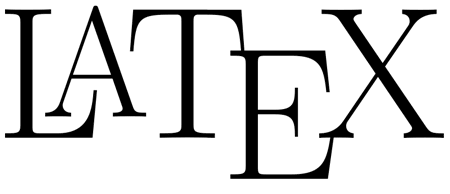
\includegraphics [scale=0.27] {latex}
 %  \caption{Подпись к картинке.} 
 %  \label{img:latex}
% \end{figure}

% Формулы в строку без номера добавляются так:
% \[ 
%   \lambda_{T_s} = K_x\frac{d{x}}{d{T_s}}, \qquad
%   \lambda_{q_s} = K_x\frac{d{x}}{d{q_s}},
% \]

\underline{\textbf{Вторая глава}}

Во второй главе мы вновь рассматриваем порождающую модель сигнала МЭГ/ЭЭГ,
чтобы на ее основе сформулировать порождающую модель матрицы кросс-спектральной плотности (кросс-спектра).
Структура порождающей модели кросс-спектра позволяет нам в явном виде указать на слагаемые, ответственные
за эффект протечки сигнала в регистрируемой записи~--- эффект, который существенно усложняет
оценку функциональной коннективности и маскирует синхронизацию с малыми фазовыми задержками.


Для удаления источников протечки сигнала мы векторизуем порождающую модель кросс-спектра и
строим оператор ортогональной проекции, который позволяет подавить вклад нежелательных
слагаемых в силу особенной пространственной структуры трех типов слагаемых, входящих
в порождающую модель кросс-спектра: слагаемых, порождающих протечку сигнала,
слагаемых, несущих информацию о взаимодействии источников с малыми фазовыми сдвигами и
слагаемых, несущих информацию о взаимодействии источников с фазовыми сдвигами, близкими к
$\pi/2$. Для описания пространственной структуры этих слагаемых мы вводим понятие 2-топографии.
Предложенная операция проекции является основной для группы методов, представленных в данной диссертации

Далее мы обобщаем операцию проекции на модели со свободной ориентацией диполя и формулируем
авторский метод поиска сетей в пространстве источников (PSIICOS).

Затем предложенный метод мы рассматриваем с точки зрения оптимальной фильтрации, вводя формальное
определение взаимной протечки сигнала для двух узлов сети в пространстве источников.
Мы получаем, что предложенная проекция порождает пространственные фильтры в
пространстве 2-топографий, которые минимизируют взаимную протечку сигнала для двух точек коры.

Построенные нами фильтры мы изучаем с точки зрения пространственной смещенности оценки
и предлагаем схему нормировки, которая приводит к несмещенной оценке. Модификацию
метода PSIICOS с такой нормировкой фильтров мы называем PSIICOS Unbiased.

Полученный таким образом метод пространственной фильтрации позволяет локализовать
сети имеющиеся сети, однако он не дает возможности отсечь ситуацию, когда
реальных взаимодействий нет. Причиной тому служит отсутствие нормировки для
оцениваемой метрики силы взаимодействия источников и как следствие невозможность выбора
объективного порога.
Чтобы справиться с этим обстоятельством, мы формулируем метод нормировки оцененных
кросс-спектральных коэффициентов с учетом эффектра протечки сигнала. Полученный
метод мы называем PSIICOS Normalized.


Чтобы справиться с эффектом протечки сигнала на уровне сетей,
мы описываем известный в литературе метод оценки со смешанной нормой,
который порождает разреженные по пространству решения,
и модифицируем его для работы в пространстве сетей с применением
предложенной проекции. Полученный метод мы называем GO-PSIICOS.


\underline{\textbf{Третья глава}}

Для валидации предложенного метода проекции в этой главе мы
сравниваем PSIICOS с набором алгоритмов, широко используемых
в нейронаучной литературе на наборе экспериментов-симуляций.
Результаты численного моделирования показывают превосходящие детекторные
характеристики PSIICOS по сравнению с остальными методами, использованными
для сравнения, в особенности для сетей с малыми фазовыми задержками.

Далее на основе симуляционных данных мы исследуем свойства метода PSIICOS.\@
В частности, мы показываем, что детекторные характеристики алгоритма действительно
показывают равномерно высокое качество решений для всего диапазона фазовых
задержек. Кроме того, мы исследуем влияние проекции на 2-топографии мнимой и действительной
частей кросс-спектра, а также протечки сигнала и показываем, что предложенная проекция
лишь незначительно ослабляет вклад действительной части, в то же время
серьезно подавляя 2-топографии протечки сигнала. Также мы исследуем влияние
ранга проекции на соотношение подавления мощностей в рассматриваемых подпространствах
и на основании этого анализа формулируем рекомендации по выбору ранга проекции.
Наконец, мы исследуем влияние неточностей прямой модели на качество решений алгоритма
PSIICOS и показываем, что для уровня шума, приближенного к реальным условиям,
качество решений падает незначительно.

Далее мы демонстрируем работу метода PSIICOS на реальных данных в
задаче воображения движения. Мы показываем, каким образом метод
может быть применен к анализу данных эксперимента и как проблема невозможности
выбора порога для метода может быть решена при помощи процедуры бутстрэпа.
Найденные на реальных данных сети мы анализируем с точки зрения физиологической
правдоподобности.

Затем мы сравниваем метод PSIICOS Unbiased с оригинальным методом,
и применяя оба метода к симуляционным данным, показываем,
что нормализация фильтров приводит к повышению качества работы алгоритма.

В следующем разделе мы иссле метод PSIICOS Normalized
и показываем, что использование нормализации для элементов кросс-спектра
позволяет отсечь найденные пары источников, которые выделяются лишь в
силу большой амплитуды, но не фазовой синхронизации.

Наконец, мы демонстрируем применение алгоритма GO-PSIIOCS и показываем,
что этот алгоритм действительно позволяет избавиться от эффекта протечки
сигнала на уровне сетей, а также способен в динамике отслеживать
возникающие и пропадающие сети.

% Можно сослаться на свои работы в автореферате. Для этого в файле
% \verb!Synopsis/setup.tex! необходимо присвоить положительное значение
% счётчику \verb!\setcounter{usefootcite}{1}!. В таком случае ссылки на
% работы других авторов будут подстрочными.
% \ifnumgreater{\value{usefootcite}}{0}{
% Изложенные в третьей главе результаты опубликованы в~\cite{vakbib1, vakbib2}.
% }{}
% Использование подстрочных ссылок внутри таблиц может вызывать проблемы.

% В \underline{\textbf{четвертой главе}} приведено описание 

В \underline{\textbf{заключении}} приведены основные результаты работы, которые заключаются в следующем:
%% Согласно ГОСТ Р 7.0.11-2011:
%% 5.3.3 В заключении диссертации излагают итоги выполненного исследования, рекомендации, перспективы дальнейшей разработки темы.
%% 9.2.3 В заключении автореферата диссертации излагают итоги данного исследования, рекомендации и перспективы дальнейшей разработки темы.

Мы описали новый метод обнаружения фазовой связности в выделенной полосе
частот, по неинвазивным данным МЭГ/ЭЭГ. Предложенный подход демонстрирует,
возможность выделять истинную линейную связь с нулевым сдвигом по фазе по
неинвазивными записям.  Это достигается за счет предложенной процедуры
проекции, работающей в пространстве сенсоров на кросс-спектральных матрицах и
позволяющей эффективно подавить вклад пространственной протечки сигнала в
действительную часть кросс-спектральной матрицы. Оказывается, что хотя
подпространство, модулируемое действительной частью исходного кросс-спектра и
подпространство, включающее мощность протечки сигнала перекрываются, достаточно
просто построить пространственный проектор, чтобы подавить большую часть
протечки сигнала.  (например, 95, см. рис. 3), и при этом сохранить
чувствительность к большинству источников с нулевой фазовой связью. Как
показано на примере численного моделирования, предлагаемая методика позволяет
сохранить чувствительность для всего диапазона значений фазового сдвига, см. рис. 9.

Используя реалистичное моделирование, мы исследовали предлагаемую методику
(PSIICOS) и сравненили ее эффективность с набором других методов, таких как
DICS, iDICS, а также методом геометрической коррекции (GCS). Метод PSIICOS
стабильно превосходил три референтных метода в обеих смоделированных конфигурациях:
как с тремя сетями с перекрывающимися профилями активности и фиксированными положениями
узлов, так и в случае симуляций Монте-Карло на широком диапазоне реалистичных
условий зашумленности, а также значений фазового сдвига.  Важно отметить, что
метод PSIICOS показал равномерное качество решений для всего диапазона средних
значений фазового сдвига.

В последние годы появилось большое количество методов обнаружения
функциональной связности.  Если бы мы имели доступ к истинным сигналам на коре,
отражающим активность каждого отдельного узла сети, то можно было бы
использовать функцию когерентности, отражающую линейную (с точки зрения теории
линейных стационарных систем) связь между сигналами.  Однако активность
корковых генераторов, измеренная неинвазивно, доступна только в виде смеси
сигналов активации из нескольких источников и, таким образом, прямое
использование сигнала сенсоров приводят к ошибочным результатам: эффект
протечки сигнала маскирует истинную функциональную связь. Для решения этой
проблемы (Nolte et al.(2004a)) предложил использовать мнимую часть
кросс-спектра в качестве статистики на уровне сенсоров, которая не чувствительна к
протечке сигнала.

Это вызвало появление ряда методов, например (Stam et al. (2007), Vinck et al.
(2011), Эвальд и др. (2014)), использующих мнимую часть кросс-спектра на уровне
сенсоров.  Хотя некоторые из них и дают преимущество перед методом imCoh, все
они не в способны обнаруживать сети с нулевой фазовой задержкой, так как мнимая
часть когеренции функционально независима от действительной части исходного
кросс-спектра в пространстве источников, который несет информацию об истинной
связности с нулевой разностью фаз. Для нулевых или близких к нулю средних
фазовых сдвигов ОСШ мнимой части кросс-спектра на уровне сенсоров недостаточно
для надежной детекции, см. рис. 9. В то же время, использование необработанной
действительной части кросс-спектра не представляется возможным из-за эффекта
пространственной протечки. Как мы показали в данной работе, использование
обратного оператора на базе LCMV для разделения данных сенсоров, как это
предлагается в методике DICS, не обеспечивает необходимой точности, а
последующее использование когерентности в пространстве
источников не позволяет получать решения удовлетворительного качества при
реалистичных значениях ОСШ.

Представленный здесь подход наиболее тесно связан со схемой геометрической
коррекции (GCS, Wens et al., 2015), первоначально введенной в применение для
анализа связи между огибающими сигналов в пространстве источников в качестве
альтернативы методам ортогонализации на основе временной структуры активации,
(Hipp et al., 2012), (Colclough et al., 2015). Подход GCS предполагает
использование топографии фиксированного узла в сочетании с фильтром на основе
обратного оператора для некоторого другого источника с которым меряется
связность фиксированного узла. Метод GCS устраняет эффект пространственной
протечки, связанный только с этим фиксированным источником.  В сравнении с этим
вместо использования топографии фиксированного источника и устранения эффекта
протечки сигнала только от него, подход PSIICOS работает в пространстве внешних
произведений топографий пар источников и предполагает создание проектора,
который учитывает вклад в протечку сигнала от всех возможных источников.
Использование сингулярного разложения позволяет построить эффективный оператор
проекции, позволяющий сконцентрировать наибольшее количество нежелательной
мощности протечки сигнала в подпространстве фиксированного ранга. Эта операция
проецирования применяется к матрице кросс-спектра в пространстве сенсоров.

Подобно GCS, PSIICOS позволяет визуализировать динамику отражающего картину
взаимодействий кросс-спектра в пространстве сенсоров и позволяет проводить анализ
в том числе не переходя в пространство источников (применение к анализу на уровне сенсоров
в данной работе не рассматривается). Например,
учитывая растущую значимость методов машинного обучения в анализе
нейрофизиологических данных, операция проекции, составляющая основу PSIICOS,
позволяет получать признаки, отражающие истинную связность в
относительно компактном пространстве сигналов на сенсорах. Проекция PSIICOS также
может быть применена к отдельным векторизованным внешним произведениям
данных на уровне сенсоров, а затем использована для обнаружения корковых участков со
значимыми корреляциями огибающих.

Как мы показали, подход с использованием порождающего уравнения позволяет
интерпретировать задачу оценки параметров порождающей модели кросс-спектра (c
ij) как стандартную недоопределенную проблему линейной регрессии,
распространенную в неинвазивных методах нейровизуализации.  Такой подход
позволяет получить четкий способ введения столь необходимой априорной
информации в задачу оценки связности. Эта информация может быть получена с
помощью диффузионной тензорной визуализации и представлена с использованием
вероятностного распределения, которое затем естественным образом используется в
рамках Байесовской парадигмы.
Менее специфичные, упрощенные априорные распределения, основанные на
пространственной разреженности, также могут быть использованы, и подход,
аналогичный описанному в (Strohmeier et al., 2016), основанный на смешанных
дробных нормах, может быть использован для построения
разреженных решателей, объясняющих наблюдаемый пространственный кросс-спектр на
уровне сенсоров активностью небольшого числа элементарных сетей в пространстве
источников.

Также, следуя по пути параметрического оценивания, можно PSIICOS позволяет применять
обобщения методов подгонки диполя, включая модифицированный алгоритм RAP-MUSIC, примененный к
матрице кросс-спектра с удаленной протечкой сигнала. Фактически, (Ewald et al. (2014)) описывает
использование MUSIC-подхода для анализа мнимой части кросс-спектра на
основе MUSIC-метрик, но, как уже отмечалось ранее, из-за использования только
мнимой части кросс-спектра, предлагаемый подход не чувствителен к сетям с
нулевыми фазовыми задержками. Кроме того, время вычисления для метода, описанного в
(Ewald et al. (2014)), велико, и авторы прибегают к двухэтапной процедуре,
чтобы избежать сканирования по $N^2$ парам источников.
Векторизованная форма кросс-спектра и соответствующее порождающее уравнение могут послужить основой
для разработки подхода RAP-MUSIC, при котором элементарные сети заменяют диполи
в исходных выкладках для этой методики (Мошер и Лихи (1999)). RAP-MUSIC
предполагает построение рекурсивных проекций от подпространства, образуемого
топографиями источников, обнаруженных на предыдущих итерациях. При применении к
векторизованному кросс-спектру для удаления обнаруженной элементарной сети,
состоящей из узлов А и В, такая проекция удалит только вклад конкретной
пары, а спроецированный кросс-спектр сохранит остальные сети, образованные источником А,
со всеми остальными источниками, за исключением узла В, а также сети, образованные источником В,
со всеми остальными источниками кроме А. Это означает, что при применении
подхода RAP-MUSIC к векторизованному кросс-спектру с удаленной протечкой сигнала мы можем
получить возможность исследовать сложные сети, состоящие более чем из одной
пары узлов. Отдельного изучения требует вопрос, решает ли эта процедура проблему, поднятую в работе
Mahjoory et al. (2017), что оценки, полученные методом бимформинга, и глобальные решения MNE
приводят к разным картинам распределения связности.

В текущей векторизованной реализации в среде MATLAB расчет проекционной матрицы
для модели пространства источников с 7000 узлами занимает менее одной секунды
расчетного времени и требует вычисления лишь одинажды для каждого испытуемого,
если предположить, что положения сенсоров фиксированы или что в данных была
сделана поправка на движения испытуемого (такая поправка возможна
использованием метода tSSS).  Векторизованная реализация сканирования по
пространству источников размером 7000 на 7000 узлов занимает полсекунды
вычислительного времени на современном ноутбуке.  Таким образом предложенный
подход является вычислительно эффективным и делает возможным проведение анализа
на основе симуляций Монте-Карло для исследования устойчивости наблюдаемых
сетей, аналогичного проведенному в данной работе.

Современные метрики взаимодействия в пространстве источников для MEG/EEG,
игнорирующие связь с нулевым сдвигом по фазе, приводят как к ложноположительным
Matias Palva и др. (2018), так и к ложноотрицательным срабатываниям. Хотя первая проблема была
решена недавно (например, Wang et al. (2018)), решение второй проблемы до сих
пор не было предложено. В этой работе мы приводим первую демонстрацию
возможности неинвазивного картирования истинной мгновенной линейной связности.
Учитывая убедительные доказательства существования такой малолатентной связи,
как это видно при инвазивных исследованиях на животных, мы полагаем, что
описанная здесь методика PSIICOS значительно расширит возможности современных
функциональных инструментов сетевого анализа.

% Strengths and limitations of PSIICOS framework

Предложенный здесь подход представляет собой новое решение для изучения
взаимодействий в данных МЭГ и может выборочно решать проблему пространственной
протечки даже в случае нулевой или близкой к нулю фазовой связности. Это
позволяет преодолеть ограничения, присущие методам, использующим мнимую часть
кросс-спектра или основанные на временной структуре данных ортогонализационные
подходы, которые по определению игнорируют нулевые фазовые взаимодействия (и
имеют слабую чувствительность к околонулевым фазовым сдвигам). Отметим, однако,
что PSIICOS требует статистической процедуры, основанной на бутстраппинге, и
что он не полностью застрахован от ложноположительных срабатываний при наличии
несвязанных источников с профилями мощности, которые значительно выше, чем у
взаимодействующих источников.

Основное внимание в данной работе мы уделяем новой проекционной схеме,
позволяющей существенно подавить вклад пространственной протечки в кросс-спектр на уровне сенсоров
и получить новое порождающее уравнение (9), позволяющее представить задачу
оценки фазовой связности как задачу оценки источника, но в пространстве пар
сигналов сенсоров. Для проведения необходимой валидации метода мы
выбрали максимально простую стратегию поиска источников для этого уравнения.
Даже при таком простом подходе к оценке наши результаты демонстрируют потенциально
более высокую производительность предлагаемой методики по сравнению с рядом
других релевантных методов и почти одинаковую чувствительность ко всему
диапазону средних значений разности фаз между временными рядами связанных
источников, включая нулевую и близкую к нулю фазовые задержки. Основываясь на
работе, описанной в работе Дарваса F (2005), мы также предложили процедуру
бутстрапа, которая может быть использована для проверки стабильности
наблюдаемого результата.

В случае наличия в данных истинной связности предлагаемая процедура бутстрапа 
имеет низкую вероятность генерации сети из пары активных, но функционально
не связанных источников, до тех пор, пока мощность этих источников
не будет существенно превышать мощность в узлах истинных сетей.
Если данные содержат несколько не связанных между собой функционально, но обладающих высокой мощностью
источников, предлагаемая процедура может привести к ложным срабатываниям. Кроме
того, учитывая описанный способ отбора сетей по верхним значениям метрики
сканирования $\rho$, мы, скорее всего, упустим некоторые истинные сети.

Лучшим способом решения обеих этих проблем является разработка эффективного
статистического теста, работающего на основе распределения для нулевой гипотезы.
Однако чтобы быть полезным, этот тест должен сохранять распределение мощности
в пространстве сенсоров, разрушая при этом нулевую и близкую к нулю
фазовую связность. Тесты, разработанные до сих пор для оценки линейной
синхронизации, в основном адаптированы к мерам, не чувствительным к мгновенной
связности. Более того, применение методов, основанных на рандомизации временных
рядов компонент ICA, не обеспечивает подходящего решения, когда необходимо
обнаружить связность с околонулевой фазовой задержкой. Для решения этих проблем необходим
подход, основанный на фазовой рандомизации источников,
которая бы уничтожала взаимные фазы, но сохраняла бы плавность фазового ответа
отдельных активаций. Однако, поскольку алгоритмы генерации суррогатных данных
соответствуют свойствам исходных данных в пространстве сенсоров (Хауфе и Эвальд 2016 г.),
то пользуясь такими методами может быть трудно отличить мгновенную корреляцию,
вызванную исключительно объемной проводимостью, от истинной связи с нулевой разностью фаз.
Поэтому необходимы более консолидированные усилия для создания надежной системы
статистического тестирования, адаптированной к методам анализа связи, таким как
описанная здесь.

Несмотря на эти ограничения, PSIICOS представляет собой первую попытку
обнаружить по данным МЭГ взаимодействие с нулевой и близкой к нулю фазовой
задержкой.  Насколько нам известно, задача оценки линейного взаимодействия на
основе MEG/EEG впервые представлена как многомерная регрессионная задача,
аналогичная той, которая встречается в классической обратной задаче для этого
типа данных. Такое рассмотрение открывает богатый спектр возможностей для
адаптации множества регуляризационных или параметрических методик,
разработанных в этой области, для решения проблемы оценки функциональной связи.

\begin{enumerate}
  \item Был проведен обзор исследований изменения функциональной коннективности
      мозга при различных паталогиях.
  \item Был разработан метод очистки данных ЭЭГ и МЭГ от протечки сигнала, на
      основе которого было разработано семейство алгоритмов оценки фазовой синхронности,
      позволяющих находить сети с близкими к нулю фазовыми задержками.
  \item Задача оценки фазовой синхронности в условиях протечки сигнала была
      сформулирована и решена как задача оптимальной фильтрации.
  \item Был предложен алгоритм, позволяющий обнаруживать сети с близкими
      к нулю фазовыми задержками, оптимальный в глобальном смысле и позволяющий
      справиться с проблемой ложноположительных срабатываний второго рода, вызванных
      протечкой сигнала.
  \item Было проведено численное исследование свойств предложенной
      проекции, показавшее, что разработанная методика позволяет
      подавить вклад подпространства протечки сигнала в оцененную
      на сенсорах матрицу кросс-спектральной плотности мощности.
  \item Численное исследование свойств метода проекции показало, что
      разработанная методика позволяет находить сети с близкими к нулю фазовыми задержками в условиях
      неинвазивных МЭГ измерений, которые характеризуются значительной протечкой
      сигнала между источниками.
  \item Сравнение с имеющимися на данный момент алгоритмами оценки коннективности
      по неинвазивным данным на основе симуляций показало значительное превосходство
      предложенной техники обнаружения сетей в условиях малых фазовых задержек.
  \item Применение метода очистки от протечки сигнала к реальным данным позволило
      обнаружить физиологически правдоподобные сети, которые невозможно обнаружить
      другими способами.
  \item Было проведенно численное исследование влияния значений ранга предложенной проекции
      на свойства алгоритма, которое позволило получить эвристику для выбора ранга.
  \item Численное исследование влияния неточностей прямой модели на качество решений
      предложенного алгоритма показало, что характерные для реальных записей
      диапазоны ошибок в оценке прямой модели слабо сказываются на качестве
      получаемых решений.
  \item Для выполнения поставленных задач был создан
      пакет утилит в среде MATLAB, в который входят средства генерации тестовых
      данных, визуализации пространственной и временной структуры сетей и наконец
      программные реализации разработанных и использованных для валидации алгоритмов.
  \item Наработки, полученные в ходе работы над данной диссертацией,
      были внедрены в пакеты программ Visbrain и Neuropycon, доступные для публичного
      использования.
\end{enumerate}



%\newpage
% При использовании пакета \verb!biblatex! список публикаций автора по теме
% диссертации формируется в разделе <<\publications>>\ файла
% \verb!../common/characteristic.tex!  при помощи команды \verb!\nocite! 

\ifdefmacro{\microtypesetup}{\microtypesetup{protrusion=false}}{} % не рекомендуется применять пакет микротипографики к автоматически генерируемому списку литературы
\ifnumequal{\value{bibliosel}}{0}{% Встроенная реализация с загрузкой файла через движок bibtex8
  \renewcommand{\bibname}{\large \authorbibtitle}
  \nocite{*}
  \insertbiblioauthor           % Подключаем Bib-базы
  %\insertbiblioother   % !!! bibtex не умеет работать с несколькими библиографиями !!!
}{% Реализация пакетом biblatex через движок biber
  \ifnumgreater{\value{usefootcite}}{0}{
%  \nocite{*} % Невидимая цитата всех работ, позволит вывести все работы автора
  \insertbiblioauthorcited      % Вывод процитированных в автореферате работ автора
  }{
  \insertbiblioauthor           % Вывод всех работ автора
%  \insertbiblioauthorgrouped    % Вывод всех работ автора, сгруппированных по источникам
%  \insertbiblioauthorimportant  % Вывод наиболее значимых работ автора (определяется в файле characteristic во второй section)
  \insertbiblioother            % Вывод списка литературы, на которую ссылались в тексте автореферата
  }
}
\ifdefmacro{\microtypesetup}{\microtypesetup{protrusion=true}}{}

